\begin{figure*}[h]
    \centering
    \begin{tabular}{c}
        \begin{minipage}{0.04\hsize}
            \centering
        \end{minipage}
        \begin{minipage}{0.24\hsize}
            \centering
            Ground Truth
        \end{minipage}
        \begin{minipage}{0.24\hsize}
            \centering
            Proposed
        \end{minipage}
        \begin{minipage}{0.24\hsize}
            \centering
            $\rm GA^2M$
        \end{minipage}
        \begin{minipage}{0.24\hsize}
            \centering
            pyGAM
        \end{minipage}
        \\ \hline
        \begin{minipage}{0.04\hsize}
            \small
            $x_0, x_1$
        \end{minipage}
        \begin{minipage}{0.24\hsize}
            \centering
            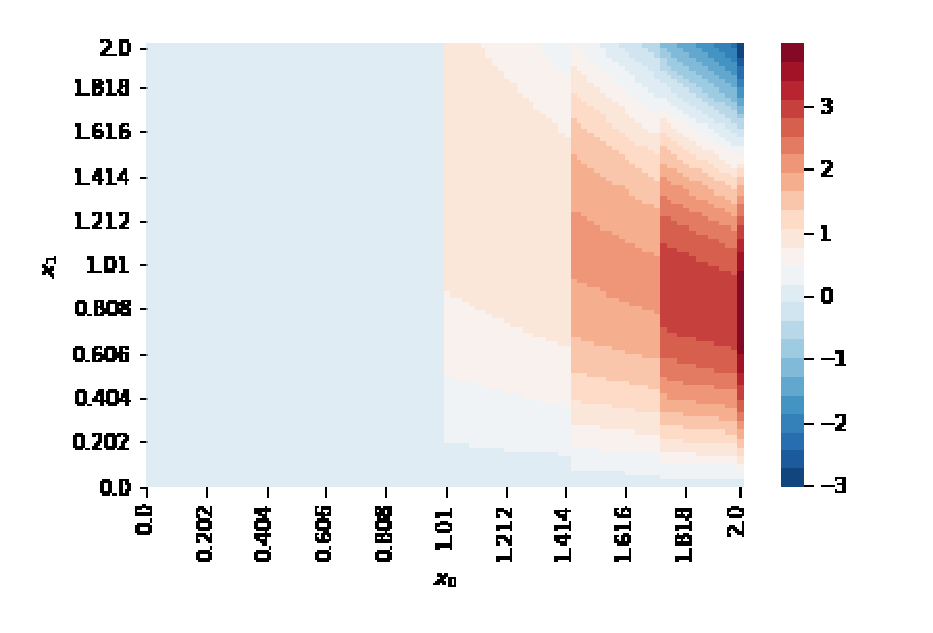
\includegraphics[width=0.95\hsize]{Matsushima/heatmaps/ideal-01.eps}
            % 理論値:$x_0 x_1$
        \end{minipage}
        \begin{minipage}{0.24\hsize}
            \centering
            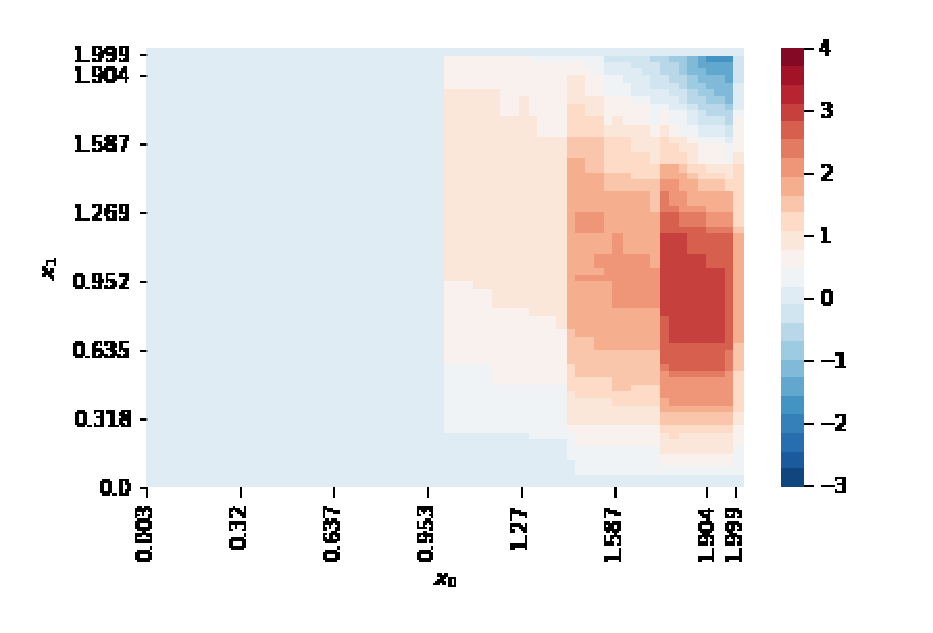
\includegraphics[width=0.95\hsize]{Matsushima/heatmaps/tvgam-01.eps}
            % IGAMの学習した相互作用
        \end{minipage}
        \begin{minipage}{0.24\hsize}
            \centering
            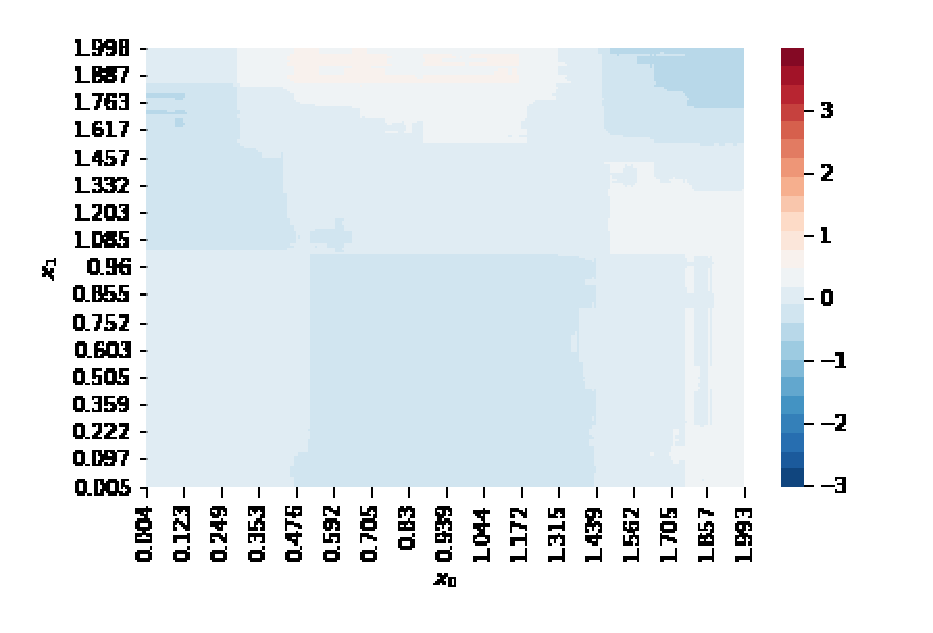
\includegraphics[width=0.95\hsize]{Matsushima/heatmaps/mltk-01.eps}
            % $\rm GA^2M$の学習した相互作用
        \end{minipage}
        \begin{minipage}{0.24\hsize}
            \centering
            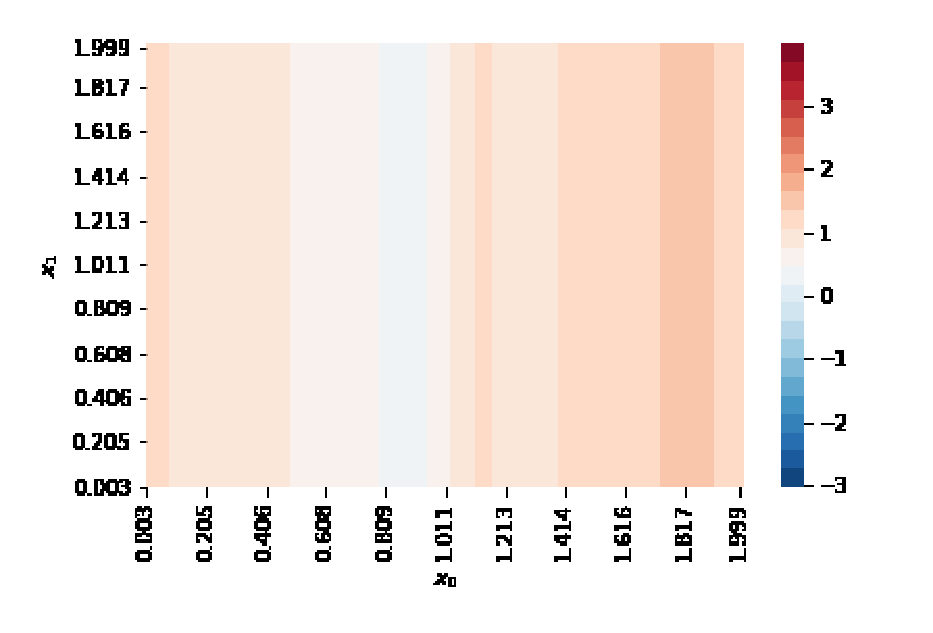
\includegraphics[width=0.95\hsize]{Matsushima/heatmaps/pygam-01.eps}
        \end{minipage}
    \end{tabular}
    \caption{人口データを用いた提案手法と既存手法($\rm GA^2M$およびpyGAM)の推定した二変数相互作用を表す関数の様子。Ground Truthは訓練データを生成した真の関数。}
\label{fig:heatmap-comparison-synthetic-data-2}
\end{figure*}